% Created 2017-01-23 Mon 09:30
% Intended LaTeX compiler: pdflatex
\documentclass[journal,10pt,compsoc]{IEEEtran}
\usepackage[utf8]{inputenc}
\usepackage[T1]{fontenc}
\usepackage{graphicx}
\usepackage{grffile}
\usepackage{longtable}
\usepackage{wrapfig}
\usepackage{rotating}
\usepackage[normalem]{ulem}
\usepackage{amsmath}
\usepackage{textcomp}
\usepackage{amssymb}
\usepackage{capt-of}
\usepackage{hyperref}
\usepackage[version=3]{mhchem}
\usepackage{minted}
\author{Willian Ver Valem Paiva}
\date{\today}
\title{Context-oriented Programming}
\hypersetup{
 pdfauthor={Willian Ver Valem Paiva},
 pdftitle={Context-oriented Programming},
 pdfkeywords={},
 pdfsubject={},
 pdfcreator={Emacs 25.1.1 (Org mode 9.0.3)}, 
 pdflang={English}}
\begin{document}

\maketitle

\section{Introduction}
\label{sec:orgf65930b}
The purpose of this study is to analyze the article \emph{Context-oriented Programming} (COP) \cite{hirschfeld2008context} 
and to show how it is viewed and used today by the community. 
For that purpose, a deep analysis of the article, and of other works related to the subject, is done, with the objective of 
well understanding the program paradigm proposed by COP. 

The contextual information is becoming the core of many contemporary applications, and the need for a support  
for context-awareness on mainstream languages has become considerable.  
As the tools offered by mainstream languages are somehow cumbersome, COP brings to the table 
this paradigm that treats of context explicitly.
For that purpose, COP uses dynamic representations of layers as \emph{first-class entities} that can be activated and deactivated in arbitrary places of the code.


The article also introduces some extensions of programming languages that have being adapted to COP :
\begin{itemize}
\item ContextL, a Common-lisp extension
\item ContextS, a Squeak/Smalltalk extension
\item ContextJ, a Java extension \cite{appeltauer2011contextj}
\end{itemize}



\section{Context definition}
\label{sec:org7e84e55}
To better define a context, COP strips it down into 3 subdivisions which are \emph{actor}, \emph{system} and \emph{environment}.
\subsection{Actor}
\label{sec:org2802b05}
\begin{center}
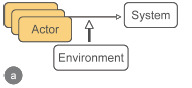
\includegraphics[width=.9\linewidth]{./actor.jpg}
\end{center}
The actor is an entity which talks with the system in such terms as: function calls, messages, and any other means that demand
a behavior from the system.
Actor-dependent behavior variants are different ways of making representations of a system or part of a system. It can be for
example the creation of different charts or graphs based on a statistical resource. The actor is the element which defines how information 
given or extracted from the system will be represented, in which form. It is part of the elements which generates the context-dependent
behavior of the system. 

The system behavior differs not only according to the different requests made by the actor
but also according to a same request made by different actors. 

\subsection{Environment}
\label{sec:orgcb9843c}
\begin{center}
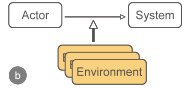
\includegraphics[width=.9\linewidth]{./environment.jpg}
\end{center}

The environment represents everything external to the relationship between \emph{actor} and \emph{system} which needs to be 
taken into consideration by the system. Some examples may be given by GPS systems, temperature sensors, accelerometer, etc \ldots{} 

A system's response to an actor's demand can be adjusted to take properties of the computational environment into account.

\subsection{System}
\label{sec:orgd54be30}
\begin{center}
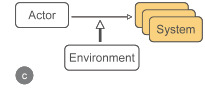
\includegraphics[width=.9\linewidth]{./system.jpg}
\end{center}

The system is a computational entity that provides some behaviors upon request. The scale of the system is not taken into consideration
here. The constituents of a system may for be example methods, objects, subsystems.

The system behavior can differ depending on its current state, on information or dependencies to other system's parts, or subsystems.    
An example of system-dependent behavior could be a notification for the change of system parts.
On the system, the determining element that has influence is the system context itself, and not any type of activity from the actors. 

\section{Structure}
\label{sec:org89133bb}
Context-oriented programming is supported by the following essential language properties : 
\begin{itemize}
\item means to specify \emph{behavioral variations}
\item means to group variations into \emph{layers}
\item dynamic \emph{activation} and \emph{deactivation} of layers based on context,
\item means to explicitly and dynamically control the \emph{scope} of layers
\end{itemize}
\cite{hirschfeld2008context} 

\subsection{behavioral variations}
\label{sec:org3f630da}


Variations consists in the addition, removal or modification of a behavior. 
Those variations can be expressed as partial definitions of modules in the underlying programming model such as procedures or classes,
but not only; variations can also be expressed as edits, wrappers or transformations.

\subsection{Activation and Deactivation}
\label{sec:orgf1e685d}


Possibility to activate or deactivate at run-time the layers bulking context-dependent behavioral variations based on the current context. 

\subsection{Scoping}
\label{sec:org51ee5d2}


Offers the control over the scope of layers that are \emph{activated} or \emph{deactivated}. These variations cam be simultaneously active or not,
within different scopes of the same running application.

\subsection{Layers}
\label{sec:org761e187}


Layers are first-class entities that group related context-dependent behavioral variations, which are being composed in reaction to contextual information.

  According to the current context, layers can be activated or deactivated. COP limits itself to the activation and deactivation of layers at run-time,
  and leave to the application the modeling of the context and the providing of what contextual information is relevant, since solutions using object-oriented
abstraction are sufficient for the task. \cite{dey2001understanding}  

\section{Multi-dimensional message dispatch}
\label{sec:org43ea783}
Multi-dimensional message dispatch \cite{smith1996simple} will be used to present COP ; but it does not mean that COP is limited to scenario. The following analogy will help understand 
that COP is the next step in the chain : procedural programming, object-oriented, and subjective programming.

\subsection{One-dimensional dispatch}
\label{sec:org9df8cc4}

\begin{center}
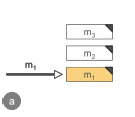
\includegraphics[width=.9\linewidth]{./one.png}
\end{center}

Also known as \emph{procedural programming} it offers only one dimension \cite{smith1996simple}. Procedures calls or names are directly linked to its implementation.
As in the image above the call to \emph{m1} can only invoke \emph{m1}.

\subsection{Two-dimensional dispatch}
\label{sec:org9055d9b}

\begin{center}
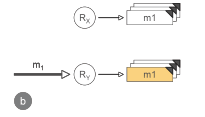
\includegraphics[width=.9\linewidth]{./two.png}
\end{center}

This refers to object-oriented programming. In this paradigm another dimension is added to the message dispatch in relation to procedural programming  \cite{smith1996simple}.
In addition to procedural programming, the message dispatch takes into consideration the receiver of the message to decide whose implementation will be used. The figure above has two receivers 
\emph{Rx} and \emph{Ry}, and each one maps to its respective implementation of \emph{m1}. A \emph{m1} call will be directed to an implementation depending on which receiver gets the message.

\subsection{Three-dimensional dispatch}
\label{sec:org30e8e0a}
\begin{center}
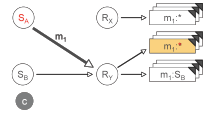
\includegraphics[width=.9\linewidth]{./three.png}
\end{center}

As introduced by Smith and Ungar \cite{smith1996simple}, subjective programming expands object-oriented programming by adding yet another dimension to the message dispatch. 
In this paradigm the implementation is not only selected by its name and receiver, but also by its sender. On the figure above, \emph{Ry} has two implementations of \emph{m1} the \emph{m1:*} 
that is a general implementation and \emph{m1:SB} which is an implementation destined to receive messages sent from \emph{SB}. In the example, the sender is \emph{SA} what makes the message 
being directed to \emph{m1:*}.

\subsection{Four-dimensional dispatch}
\label{sec:org4065866}
\begin{center}
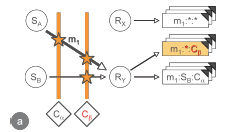
\includegraphics[width=.9\linewidth]{./four1.png}
\end{center}
\begin{center}
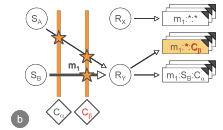
\includegraphics[width=.9\linewidth]{./four2.png}
\end{center}
   By adding one more dimension to the message dispatch ("\emph{context}"), context-oriented language takes subjective programming a step further, by taking the context into consideration 
when selecting a method's implementation.

For example on the figures above we have two possibilities. As already seen in subjective programming which takes into consideration the senders \emph{SA} and \emph{SB}, in this situation,
two new elements \emph{Ca} and \emph{Cb} are added ; those are the context. And sender \emph{SA} is affected by both contexts  \emph{Ca} and \emph{Cb} ; and \emph{SB} is only affected by the context \emph{Cb}. For that reason 
when the call is made from sender \emph{SA} in the "\emph{figure a}" the implementation to be used is the \emph{m1:*:Cb} as its signature fits the call received "\emph{m1:SA:Ca:Cb}". 
On the second figure, "\emph{figure b}", the sender is \emph{SB} ; in this case the call signature is \emph{m1:SB:Cb} which also fits for the method  \emph{m1:*:Cb}.

\section{Examples}
\label{sec:org905a739}
In this section, we will present brief examples of contextJ \footnote{At the time when this text is being written, contextJ is not being maintained any more, but of its features can be found on its successor \emph{jcop} \url{https://www.hpi.uni-potsdam.de/hirschfeld/trac/Cop/wiki/JCop}} \cite{appeltauer2011contextj} 
to show context-oriented programming in action.

Obs: the contextJ code showed on the following samples are a proof of concept. To achieve such functionalities 
a rework on the Java from the compiler to the virtual machine itself would be necessary. 

Here are presented at first the definition of two classes ; one to represent a Person that has a name, address and employer ; and a second 
class to represent an Employer that also has a name and address.
Both classes have the \emph{toString} method implemented. This method just prints the name of the object like = Name: name =. 
On the \emph{Person class} two layers are created \emph{Address} and \emph{Employment} which are the \emph{first-class} entities, used, in this case, to
override the method \emph{toString}. 

Note the use of \emph{proceed}, used to ensure that the original implementation of the method is called, in a way similar to that of the
\emph{super} in Java.

\begin{minted}[frame=lines,fontsize=\scriptsize]{java}
class Person{

    private String name;
    private String address;
    private Employer employer;

    Person(String newName,
           String newAddress,
           Employer newEmployer){

        this.name = newName;
        this.address = newAddress;
        this.employer = newEmployer;

    }

    String toString(){
        return "Name: "+name;
    }

    layer Address {
        string toString(){
            return proceed()+
                "; address: "+
                address;
        }
    }

    layer Employment {
        string toString(){
            return proceed()+
                "; [Employer] "+
                employer;
        }
    }

}

class Employer{
    private String name;
    private String address;

    Employer(String newName,
             String newAddress){

        this.name = newName;
        this.address = newAddress;
    }

    String toString(){
        return "Name: "+name;
    }

    layer Address {
        string toString(){
            return proceed()+
                "; address: "+
                address;
        }
    }

}
}
\end{minted}

Now, to use those layers, contextJ provides \emph{with} and \emph{without} for their activation and deactivation,
example:

\begin{minted}[frame=lines,fontsize=\scriptsize]{java}
Employer vub = new Employer("VUB","1050 Brussel");

Person somePersom = new Person("Pascal Costanza",
                               "1000 Brussel",
                                vub);

with(Address){

    with(Employment){
        System.out.printls(somePersom);
    }

}
\end{minted}
Note the possibility to chain and nest the layers activation to get the desired result :    

\begin{verbatim}
Output:
 Name: Pascal Costanza; Address: 1000 Brussel;
 [Employer] Name: VUB; Address: 1050 Brussel
\end{verbatim}

When looking at this example, it is possible to see the similarity of the layers with the design pattern \emph{decorator}, where you can nest functionalities into
the original object. Somehow, the layers approach presented by COP has its elegance, and simplifies the code. But as the layers have to be declared on the class,
it gets behind \emph{decorator} since a new decoration can be created at run-time. On the other hand, the advantage of COP over the \emph{decorator} is the use of \emph{with} and \emph{without} that makes
it easier and simple the control of the activation and deactivation of a functionality.

\section{Related Work}
\label{sec:org8ebe63d}

\emph{Context-oriented programming} share a bit of the design with \emph{Aspect-oriented programming} (AOP) \cite{kiczales1997aspect} and \emph{Feature-oriented programming} (FOP) \cite{prehofer1997feature}.


Aspect-oriented programming paradigm introduces the means to modulate \emph{crosscutting concerns} and decrease code scattering. On the other hand, feature-oriented programming also tackles the 
\emph{crosscutting concerns}.

In their own way, both paradigms engage on diminishing the cumbersomeness of dealing with \emph{crosscutting concerns} in the actual scenario of object-oriented programming.


When looking at FOP and the mixing layers approach \cite{smaragdakis2002mixin}, it has a noticeable similarity to the layers on COP, but the difference among those paradigms lies
in the fact that FOP is focused on the compile-time and COP introduces a dynamic activation and deactivation of layers at run-time.

\section{Discussion}
\label{sec:org334ba5c}
As was made clear, how to deal with \emph{crosscutting concern} has being a dilemma for the programming community and many techniques to deal with such a riddle have been elaborated.

Each technique has been accepted differently by the community. This goes from some bad techniques such the anti-pattern \emph{Grand central station}, where every significant method of function
passes through a monstrous subroutine, to the elaborate and well thought solutions such as many of the creational design patterns, namely \emph{decorator} and  \emph{compositor}.
And it even went to, as COP shows it, the complete rethinking of the paradigm used to program, and pushing further from object-oriented, with the aim to make it possible to deal 
with \emph{crosscutting concerns} in a cleaner and more elegant way.

What COP brings to the table has a full potential for being a game change on the software architecture design, but yet it has not been really embraced and accepted. On the other hand,
Aspect-oriented programming had a large acceptance, and has even been integrated in many of the mainstream languages like \emph{C++}, \emph{Java}, \emph{Scala} and some others. It has also been integrated
into some big well known frameworks like \emph{Spring} for java.

We can then conclude that, even if COP has shown some qualities and value, it does not seem mature enough to be integrated in mainstream programming. 








\bibliographystyle{unsrt}
\bibliography{../../.spacemacs.d/bib/references}
\end{document}